% THIS IS SIGPROC-SP.TEX - VERSION 3.1
% WORKS WITH V3.2SP OF ACM_PROC_ARTICLE-SP.CLS
% APRIL 2009
%
% It is an example file showing how to use the 'acm_proc_article-sp.cls' V3.2SP
% LaTeX2e document class file for Conference Proceedings submissions.
% ----------------------------------------------------------------------------------------------------------------
% This .tex file (and associated .cls V3.2SP) *DOES NOT* produce:
%       1) The Permission Statement
%       2) The Conference (location) Info information
%       3) The Copyright Line with ACM data
%       4) Page numbering
% ---------------------------------------------------------------------------------------------------------------
% It is an example which *does* use the .bib file (from which the .bbl file
% is produced).
% REMEMBER HOWEVER: After having produced the .bbl file,
% and prior to final submission,
% you need to 'insert'  your .bbl file into your source .tex file so as to provide
% ONE 'self-contained' source file.
%
% Questions regarding SIGS should be sent to
% Adrienne Griscti ---> griscti@acm.org
%
% Questions/suggestions regarding the guidelines, .tex and .cls files, etc. to
% Gerald Murray ---> murray@hq.acm.org
%
% For tracking purposes - this is V3.1SP - APRIL 2009

\documentclass{acm_proc_article-sp}

\usepackage{algorithm}
\usepackage{algpseudocode}
\usepackage{gensymb}

\begin{document}

\title{Paralellization of a genetic algorithm training framework}
%
% You need the command \numberofauthors to handle the 'placement
% and alignment' of the authors beneath the title.
%
% For aesthetic reasons, we recommend 'three authors at a time'
% i.e. three 'name/affiliation blocks' be placed beneath the title.
%
% NOTE: You are NOT restricted in how many 'rows' of
% "name/affiliations" may appear. We just ask that you restrict
% the number of 'columns' to three.
%
% Because of the available 'opening page real-estate'
% we ask you to refrain from putting more than six authors
% (two rows with three columns) beneath the article title.
% More than six makes the first-page appear very cluttered indeed.
%
% Use the \alignauthor commands to handle the names
% and affiliations for an 'aesthetic maximum' of six authors.
% Add names, affiliations, addresses for
% the seventh etc. author(s) as the argument for the
% \additionalauthors command.
% These 'additional authors' will be output/set for you
% without further effort on your part as the last section in
% the body of your article BEFORE References or any Appendices.

\numberofauthors{2} %  in this sample file, there are a *total*
% of EIGHT authors. SIX appear on the 'first-page' (for formatting
% reasons) and the remaining two appear in the \additionalauthors section.
%
\author{
% You can go ahead and credit any number of authors here,
% e.g. one 'row of three' or two rows (consisting of one row of three
% and a second row of one, two or three).
%
% The command \alignauthor (no curly braces needed) should
% precede each author name, affiliation/snail-mail address and
% e-mail address. Additionally, tag each line of
% affiliation/address with \affaddr, and tag the
% e-mail address with \email.
%
% 1st. author
\alignauthor
Alex Peyrard\\
       \affaddr{J114030904}\\
       \email{alex.peyrard@gmail.com}
% 2nd. author
\alignauthor
Thierry Cantenot\\
       \affaddr{J114030901}\\
       \email{thierrycantenot@gmail.com}
}
% There's nothing stopping you putting the seventh, eighth, etc.
% author on the opening page (as the 'third row') but we ask,
% for aesthetic reasons that you place these 'additional authors'
% in the \additional authors block, viz.
\date{\today}
% Just remember to make sure that the TOTAL number of authors
% is the number that will appear on the first page PLUS the
% number that will appear in the \additionalauthors section.

\maketitle

\begin{abstract}
This paper is the report for the parallel computing project of Thierry Cantenot and Alex Peyrard, group 2, for the parallel computing course of Shanghai Jiaotong University, spring semester 2015.

The project consists in parallelization of a genetic algorithm training framework. In the first part we will talk about what is a genetic algorithm. We will then analyze which parts of a genetic algorithm can be parallelized to gain efficiency. We will then explain how we used a genetic algorithm framework to solve a small 2D physics game where we train cars to avoid obstacles and go to a destination point. At last, we will analyze the results we obtained.
\end{abstract}

\keywords{Genetic algorithm, Parallel computing} % NOT required for Proceedings

\section{Genetic algorithms}
A genetic algorithm is an algorithm of reinforcement learning that uses a process inspired from real-life evolution in species to train individuals of a population to solve a problem.

In a genetic algorithm, a problem needs to be solved by an individual, which has a set of parameters that can vary. The goal is to find the set of parameters that allow to solve the problem best. To do this, we require a fitness function that will give us an evaluation of the individual. The more the fitness of an individual is good, the better it is at solving the problem.

Each of the varying parameters is called a gene, and individuals are sometime called phenotype, to parallel real-life genetics.

At first, we create a population. It is a set of $N$ individuals, with random genes. We call this population generation 0. This population will then train, or evolve, according to a few principles.

Every generation, we compute the fitness of every individual.
We then produce the next generation by several methods :
\begin{itemize}
	\item Crossover
	\item Mutation
	\item Elitism
\end{itemize}

Lets now explain each of those methods.
\subsection{Crossover}
Crossover mimics the reproduction process of real-life evolution. Two individuals, called parents, are selected from the previous generation. This selection can happen with different means but should comply to the survival of the fittest rule which is that the fittest individuals have a highest probability of reproducing, thus of being selected. Nevertheless, every individual should have a probability, albeit small for individuals with low fitness, of being selected. This allows to keep variety in the genes. A popular selections scheme is the lottery, in which probability is proportional to fitness. Another is to rank individuals by fitness and then have the probability be proportional to rank.

Those two parents are then used to create a child individual, whose genes are randomly taken from a parent. A scheme is to order genes, randomly choose a midpoint, and then copy all of genes inferior to the midpoint from parent 1, and all others from parent 2.
Another scheme is to, for each gene, choose a parent randomly with a 50\% chance and copy the gene from that parent.

The child is then added to the population of the next generation, and the process is repeated as many times as necessary until the next generation's population is the same size as the previous one.

This creates new individuals by mixing genes of the previous generation, and favours genes coming from high-fitness individuals.

\subsection{Mutation}
Mutation mimics another real-life effect. The mutation follows a probability called mutation rate. Each gene of a newly created individual (created by crossover) has a probability equal to the mutation rate of mutating. Mutating randomly changes its value, either by replacing it with a new value or by adding or substracting a random value to it. This allows genes with values that weren't in the original population  to appear in a later population. In practice, mutation rate should be high enough to produce new genes and keep variety in the gene pool, but low enough to allow bad genes of disappearing from the gene pool. It usually lies between 1\% and 10\%.

\subsection{Elitism}
Elitism is an optional parameter. When applying elitism, the elitism parameter is an integer, usually small. It allows a small number of the best individuals to be copied from the previous generation to the next one, without crossover and mutation, and before creating the rest of the population with crossover. This allows us to be sure to keep the bests individuals.

After those three methods are used to create the new generation, the new population has it fitness computed, and the whole process is repeated for the desired amount of time, or until the desired fitness is attained.


\section{Parallelization of the genetic algorithm}
This algorithm can be very efficiently parallelized. First, the fitness computation of every individual is embarassingly parallelizable. We can evaluate each individuals fitness in parallel. This means that we can create a pool of workers and a queue of individuals, and each worker will take an individual from the queue, evaluate it, and do it again until the queue is empty. This scheme is very interesting when the time necessary to evaluate one individual can vary. Another scheme, for interesting if we know that the evaluation time is identical for every individual, would be to simply assign to each thread the number of individuals divided by the number of threads individuals, and to try to have a population size equal to a multiple of the number of threads to avoid wasting time.

Parallelization can also be included in the crossover and mutation steps. But those steps should always have the same time needed by individual, thus it is best to use the second one of the two schemes described.

During crossover and mutation, it also could be possible to parallelize the crossover and mutation over the genes, but it is actually more efficient to parallelize across the individuals in the first place, because it has no dependency over shared data, and thus less overhead.

\section{Our problem}
To test our genetic algorithm framework, we coded a small game in which a car in a 2D top down view can move by accelerating forward and backward and steer. Obstacles are randomly added to the world the cars can move in. A destination point is chosen, and the car should move toward the destination. Thus our fitness function is inversely proportionate to the distance from the car to the destination. If the car touches an obstacle, it dies and the simulation stops here. It is thus better for the car to learn to avoid the obstacles.

The car is controlled by a neural network. The inputs of the neural network are the angle between the car and the destination (rounded to the nearest 90$\degree$ to only give a sense of direction and avoid overfitting) and a set of distances to detected obstacles in several directions from the car. The car can thus detect obstacles.
The angle of detection are parametrisable, in our case we detect obstacles at angles of 0$\degree$, -90$\degree$, 90$\degree$, 45$\degree$, -45$\degree$, 22.5$\degree$ -22.5$\degree$, 67.5$\degree$, -67.5$\degree$ and 180$\degree$ from the car. It can thus more easily detect obstacles in front of it.

The outputs of the neural network are the controls : Accelerate forward, accelerate backwards, steer left and steer right.

The genes of our individuals are the weights of the neural network. All others parameters of our cars are not variable. Thus the only thing that can change is the neural network, thus the AI of the car.

We then used our framework to solve this problem with parallel computing.

\begin{figure}[!htbp]
\centering
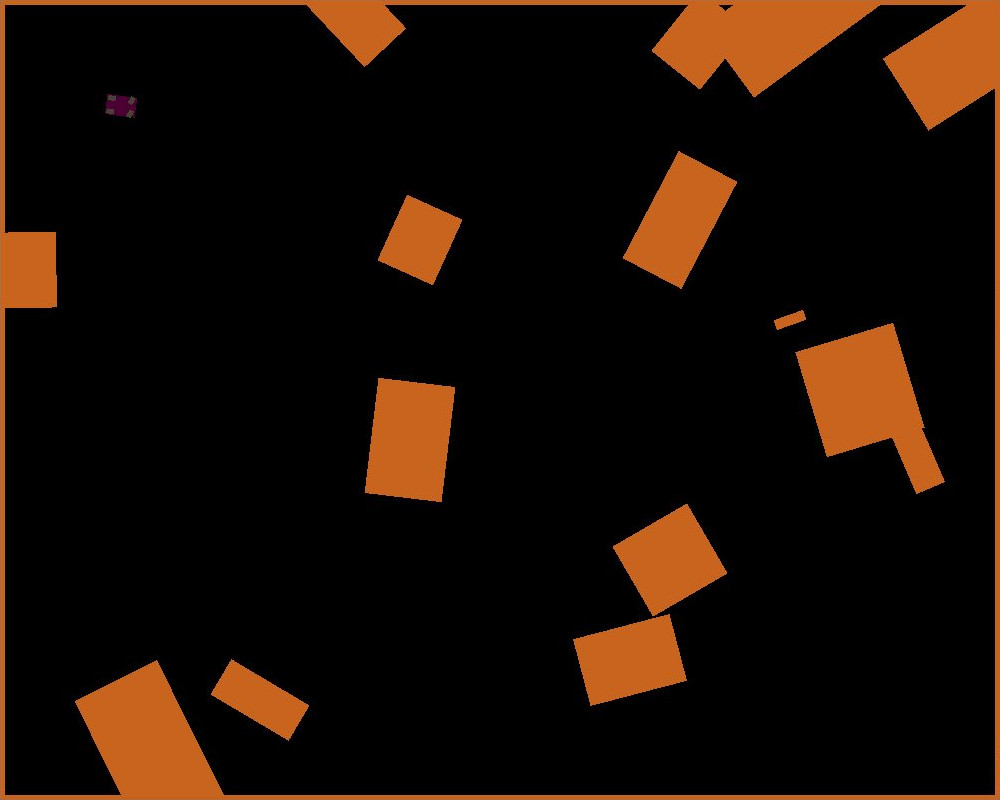
\includegraphics[width=\linewidth]{./images/cars.jpg}
\caption{Our car simulation}
\label{fig1}
\end{figure}

On figure \ref{fig1} you can see the car in the top left corner, currently steering to its left. The orange boxes are obstacles.

\section{Coding the framework}

The framework, implemented in C++11, consists of three separate components: a neural network module, a genetic algorithm framework and a physics component for the cars.\\
All of these three components have been coded from scratch, except the physics simulation which relies on the physics engine Box2D\footnote{http://box2d.org/}. \\

\noindent
The parallelization is performed exclusively with OpenMP. The main reason is that the training of neural networks with  a genetic algorithm is embarassingly parallel: there is no need for communications. \\

\noindent
The parallelization is done in two parts:
\begin{itemize}
	\item The matrix multiplications, used in the feed forward  algorithm for example, can be parallelized with OpenMP.
	\item The evolution performed by the genetic algorithm
\end{itemize}
\textit{Note:} In our case, the parallelization of the matrix multiplications is disabled because the matrix size are too small; and the computation time would be dominated by the creation of the thread pool. However the implementation has been written\footnote{See matrix.inl}. \\

The main source source of parallelism is found in the core of the evolution algorithm\footnote{See evolution.inl}.
\begin{algorithm}
\begin{algorithmic}[1]
    \For{each generation}
        \State

        \State \textit{\small{// Parallel section for OpenMP}}
        \For{each individual}
            \State compute fitness of individual
        \EndFor

        \State

        \State \textit{\small{// Parallel reduction(:+) operation with OpenMP}}
        \State Compute cumulative fitness

        \State

        \State \textit{\small{// Parallel section for OpenMP}}
        \State \textit{\small{// Create mating pool}}
        \For{each individual}
            \State compute relative fitness
        \EndFor

        \State

        \State \textit{\small{// Serial section}}
        \State \textit{\small{// Initialize mating pool}}
        \State sort by decreasing relative fitness and compute scores

        \State

        \State \textit{\small{// Parallel section for OpenMP}}
        \For{each new\_individual}
       		\State $p_1 \gets selectParent()$
       		\State $p_2 \gets selectParent()$
            \State new\_individual $\gets$ crossover($p_1$, $p_2$)
            \State mutate(new\_individual)
            \State add to next generation
        \EndFor

        \State

        \State generation $\gets$ next\_generation

        \State
    \EndFor
\end{algorithmic}
\end{algorithm}



\section{Conclusions}

%\end{document}  % This is where a 'short' article might terminate

%ACKNOWLEDGMENTS are optional


%
% The following two commands are all you need in the
% initial runs of your .tex file to
% produce the bibliography for the citations in your paper.
\bibliographystyle{abbrv}
\bibliography{sigproc}  % sigproc.bib is the name of the Bibliography in this case
% You must have a proper ".bib" file
%  and remember to run:
% latex bibtex latex latex
% to resolve all references
%
% ACM needs 'a single self-contained file'!
%
%APPENDICES are optional
%\balancecolumns

\subsection{References}
Generated by bibtex from your ~.bib file.  Run latex,
then bibtex, then latex twice (to resolve references)
to create the ~.bbl file.  Insert that ~.bbl file into
the .tex source file and comment out
the command \texttt{{\char'134}thebibliography}.
% This next section command marks the start of
% Appendix B, and does not continue the present hierarchy

\end{document}
